\documentclass[a4paper, 10pt,]{article}
\usepackage[english, russian]{babel}
\usepackage[T2A]{fontenc}
\usepackage[utf8]{inputenc}
\usepackage{lipsum}
\usepackage{enumitem}
\newcommand{\RomanNumeralCaps}[1]
    {\MakeUppercase{\romannumeral #1}}
\usepackage[colorlinks, linkcolor=blue]{hyperref}
\usepackage{graphicx}
\usepackage{setspace}
\usepackage{geometry}
\geometry{top=18mm}
\geometry{bottom=18mm}
\geometry{right=15mm}
\geometry{left=15mm}
\usepackage{multicol}
\usepackage{wrapfig}
\setlength{\parindent}{0.5cm}
\setlength{\parskip}{0.2cm} 
\setlength{\columnsep}{0.5cm}
\graphicspath{{images/}}

\usepackage{titlesec}\titleformat{\subsection}
  {\textit\normalsize} % Обычный шрифт, нормальный размер 
  {\thesection}{1em}{}
  \usepackage{titlesec}\titleformat{\section}
  {\textit\normalsize\centering} % Обычный шрифт, нормальный размер 
  {\thesection}{1em}{}
\setcounter{page}{231} % нумерация страниц


\begin{document}
\multicols{2}

\section*{\uppercase\expandafter{\romannumeral 2}. Proposed approach}
\hspace{0.5cm} In the development of the module of building plans
for solving the problems of the IS, it is proposed to
use the OSTIS Technology, focused on the development
of a class of systems, which are called knowledgemanaged computer systems, as well as its basic principles
[21], since any \textit{ostis-system} consists of \textit{knowledge base,
problem solver} and \textit{user interface}, which corresponds to
the classical definition of an IS [22].

This technology uses a unified semantic network with
a set-theoretic interpretation as a formal basis for knowledge representation. This representation model is called
SC-code (Semantic computer code). Elements of such
semantic network are called sc-nodes and sc-connectors
(sc-arc, sc-edges). Agents in the developed system described by means of SC-code will be called a semantic
agent or simply sc-agent.

As it was mentioned earlier, in order to be able to
solve some non-trivial problems it is necessary to be able
to divide them into trivial ones, i.e. to build a plan for
problem solving. When constructing plans for solving
the problem of an IDS, it is suggested to divide the main
problem into separate subproblems taking into account
various separate independent components necessary for
solving the main problem.

Let us introduce the concepts \textit{problem, subproblem,
action, subaction}.

\subsection*{\textit{A. Fragment of the obtained ontology}}

\paragraph{\textbf{\textit{planning of IDS problems}}}
\hfill\break:= [partitioning a problem into smaller problems - allocation of separate subproblems for solving the main
problem]

The concept of \textbf{problem} is directly related to the
concept of \textbf{action}, so let’s consider the classification of
the concept of \textbf{action}.

1 \textit{action classification:} Let us consider the specification of the concept of \textit{action} in SCn code.
\paragraph{\textit{action}} 

\hfill\break:= [\textit{impact}, in which the \textit{subject'} carries out the \textit{action}
purposefully, i.e. according to some \textin{target*}]
\hfill\break:= [targeted action performed by one or more actors
(cybernetic systems) with the possible application
of some tools]
\paragraph{\subset \textit{impact}}
\hfill\break:= [a process in which at least one influencing entity
(subject of influence ') and at least one entity
to be influenced (object of influence ') can be
clearly distinguished]
\paragraph{\subset \textit{process}}
\hfill\break:= [a purposeful ("conscious") process performed (controlled, realized) by a certain subject]
\hfill\break:= [work]
\hfill\break:= [problem solving process]
\hfill\break:= [target-oriented process]
\hfill\break:= [holistic piece of some activity]
\hfill\break:= [A purposeful process controlled by some entity]
\hfill\break:= [the process of performing some action by some
subject (executor) on some objects]
\paragraph{\textbf{\textit{target*}}}
\hfill\break:= [target situation*]

\paragraph{\subset \textit{specification}}
\hfill\break:= [description of what is to be obtained (what situation
is to be achieved) as a result of performing a given
(specified) action*]
Each \textit{action} performed by one or another \textit{subject} is
interpreted as a process of solving a certain problem,
i.e., a process of achieving a given \textit{target*} under given
conditions, and, therefore, is performed purposefully.
However, an explicit indication of the \textit{action} and its relation to a particular \textit{problem} may not always be present
in memory. Some problems may be solved by certain
subjects permanently, e.g., optimizing a knowledge base,
searching for incorrectness, etc., and for such problems
it is not always necessary to explicitly introduce the
\textit{structure} that is the formulation of the \textit{problem}.

In its turn, the concept of a \textit{subproblem} or \textit{action}
is a separate independent \textit{problem} (action), which is
performed within the framework of some other extensive
\textit{problem} (action).

\subsection*{\textit{B. Architecture of a problem solver for partitioning problems into subproblems}}
To realize an IS, which includes methods and means
of constructing plans for solving problems of the IS, it
was necessary to build a decomposition of the problem
solver of the system, where the key agent of the IS is an
abstract non-atomic sc-agent of constructing a plan for
solving problems of the IS, taking into account the above
classification.

The following is the decomposition of the IS problem
solver in the form of SCn-code:
\paragraph{\textbf{\textit{Problem solver for partitioning a problem into
subproblems of an intelligent system}}}

\hfill\break${\Rightarrow}$
\textit{decomposition of abstract sc-agent*:}

\begin{itemize}
\item [\{ $\bullet$] Abstract sc-agent for classifying a message by topic
\\${\Rightarrow}$ 
\textit{realization*:}

\hspace{0.5cm}C++ language 

\item Abstract sc-agent for classifying a message by type
\\${\Rightarrow}$ 
\textit{realization*:}

\hspace{0.5cm}C++ language 
\item Abstract sc-agent for generating a problem condition from a template
\\${\Rightarrow}$ 
\textit{realization*:}

\hspace{0.5cm}C++ language 
\item Abstract sc-agent for finding the meaning of a problem
\\${\Rightarrow}$
\textit{realization*:}

\hspace{0.5cm}C++ 
\item Abstract sc-agent targeting
\\${\Rightarrow}$
\textit{realization*:}

\hspace{0.5cm}C++ language 
\item Abstract non-atomic sc-agent for constructing a problem-solving plan for an intelligent dialog system
\\${\Rightarrow}$
\textit{realization*:}

\hspace{0.5cm}C++ language 
\item Abstract sc-agent for knowledge base replenishment
\\${\Rightarrow}$
\textit{realization*:}

\hspace{0.5cm}C++ language 
\item Abstract sc-agent for generating a response to a message 
\\${\Rightarrow}$
\textit{realization*:}

\hspace{0.5cm}C++ language
\item [\}] 
\end{itemize}


In this article we consider the approach to solving complex problems, so we will consider in detail the abstract non-atomic sc-agent of building a plan for solving problems of the IS.

As a part of the abstract non-atomic sc-agent of constructing a plan for solving problems of an intelligent dialog system, the following group of agents that break the problem into separate subproblems was identified:
\paragraph{\textbf{\textit{Abstract non-atomic sc-agent for constructing a plan for solving problems of an intelligent system}}}

\hfill\break${\Rightarrow}$
\textit{decomposition of abstract sc-agent*:}

\begin{itemize}
\item [\{ $\bullet$] Abstract sc-agent for solving a composite problem

\\${\Rightarrow}$ 
\textit{realization*:}

\hspace{0.5cm}C++ language 

\item Abstract non-atomic sc-agent for solving a
simple problem

\\${\Rightarrow}$ 
\textit{realization*:}

\hspace{0.5cm}C++ language 
\item [\}] 
\end{itemize}


\subsection*{\textit{C. Principles of application of the developed solver in application systems}} 
The approach proposes the introduction of separate modules with their ontologies and problem solvers into the developed system, which will increase the range of capabilities of the developed system.

Let us consider \textit{abstract non-atomic sc-agent of constructing a plan for solving problems of an IS} on the example of a system with implemented module of an IS on geometry.

Examples will be considered on the basis of dialog-based ISs.

The abstract sc-agent for solving a composite problem takes as input one parameter, which specif i es the condition of the composite problem written in the form of sc-code and a node denoting the target of solving the problem. The task of this agent is to divide the original problem into simple subproblems, and also to call for each simple subproblem one of the agents for solving simple problems in a certain sequence, which is set by the abstract sc-agent of the interpretation of non-atomic action, in some cases there is a need to execute the agent of the application of the logical formula [23]. The result of solving the subproblem is recorded in the decision tree, which is ultimately the solution of the user’s problem.

That is, the abstract non-atomic sc-agent of constructing a plan for solving the problems of the IS involves breaking the main problem-request into separate subproblems to form a better response to the user’s message, i.e., solving smaller problems allows increasing the quality of knowledge immersed in the database. As an input construct, we obtain a situation that is formed due to an abstract sc-agent of target-setting developed within the framework of the IS under development, the input of which is a user’s user’s message. As an example, let us take the user’s request "What is the area of the figure?".

Depending on the knowledge in the KB, the formed target may not be deployed at all, or it may be more deployed, which allows to break the problem into sub-problems more qualitatively, i.e., to solve the problem in the most accurate way in the future.

The figure \pageref {fig:picture}  shows an example of a more extended generated situation, namely the target of "find out the area of a figure".

When receiving a question from a user about the area of a figure without additional instructions, it is impossible to answer it directly. As a result of the abstract target-setting agent’s work in the IS, a situation arises that requires solving a non-trivial problem. To break this problem into simpler subproblems, an abstract non-atomic sc-agent of constructing a problem-solving plan is used.

We apply a depth-first search method over a graph in which we define the corresponding subproblems that are trivial. Unknown values for these subproblems can be discovered by searching the KB or by using an agent included in the IS module on geometry. If it is still not possible to solve the problem, we ask for clarifications from the user to obtain additional information that will contribute to expanding the description about the situation.

{
    \centering
    \includegraphics[width=0.9\linewidth]{images/picture.png}
    \caption{\footnotesize Figure 1. Example of a detailed situation generated as a result of a
dialog with a user}
    \label{fig:picture}
}

Therefore, the agent of building a plan for solving problems of the IS in turn consists of an agent for solving a composite problem and an agent for solving a simple problem. That is, in the context of the developed dialog system, a simple problem will be an indivisible problem that does not require additional information, such a problem, the result of which can be solved as a result of a search in the KB, or as a result of the work of an abstract sc-agent from additional implemented modules.

In general, a \textit{problem solving plan} consists of a sequence of simple and compound problems. The composite problems are solved by \textit{Abstract sc-agent for interpreting non-atomic action.} It receives 1) a processing pro-gram in the form of a template and 2) sets of arguments that it retrieves from the semantic neighborhood of the composite problem. The template data is matched with the arguments and the corresponding agents are invoked, to solve the atomic actions belonging to the composite problem. The invoked agents perform the actions of the composite problem.

In essence, this agent is an interpreter that generates a processing program, i.e., a program that includes a sequence of agent executions. A processing program — is a description of a non-atomic action to be performed to solve a composite problem. Sequential execution of agents is produced by sequential processing of transitions between agents.

The transition to the next action depends on the result of the previous one. After the action is completed, i.e.
after it is added to the problem executed class, its success is checked to determine the required transition. There are 3 variants of transition:
\begin{enumerate}
 \item[1] Transition on successful completion of the action.

{
    \centering
    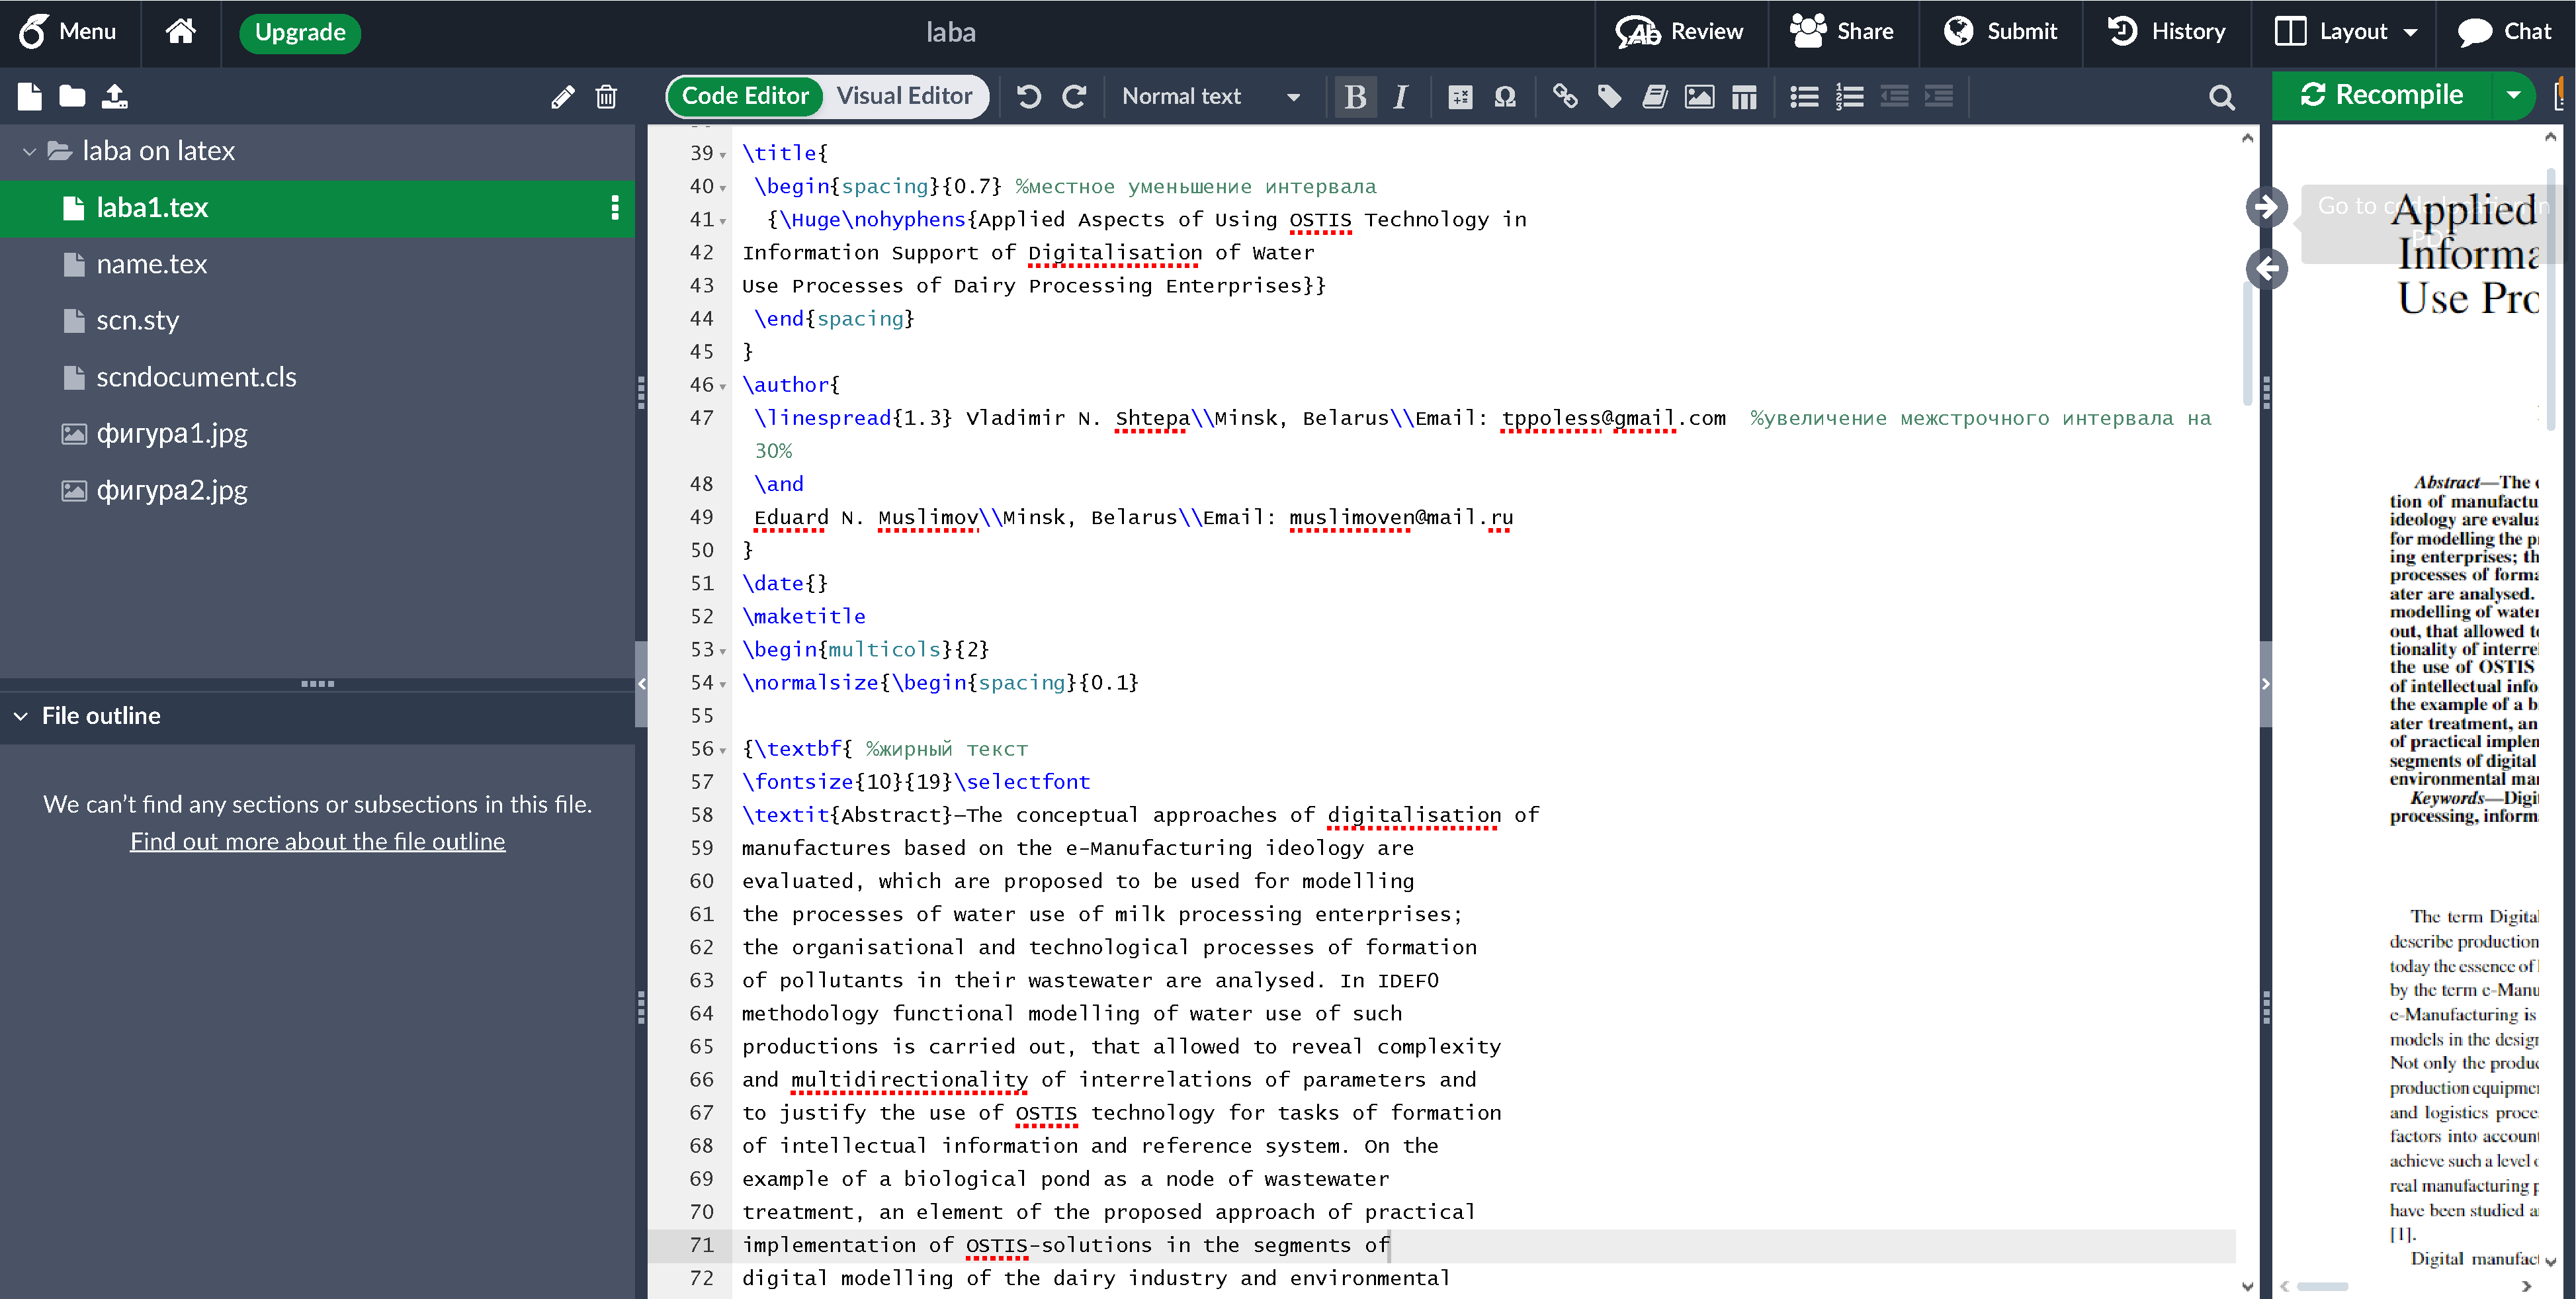
\includegraphics[width=1\linewidth]{images/picture2.png}
    \caption{\footnotesize Figure 2. An example of recording a transition between two actions,
depending on the result of the previous action}
    \label{fig:picture2}
}

 It is defined by the then* relation. Transition by this relation is performed at successful completion of the action from which the transition is performed (its addition to the class of successfully completed action).

\item[2] Transition at unsuccessful completion of the action.
It is set by the then* relation. The transition by this relation is performed at the successful completion of the action from which the transition is performed (its addition to the class of unsuccessfully completed action).

\item[3] Unconditional transition.
\end{enumerate}
The figure \pageref {fig:picture2} shows an example of recording a transition between two actions, depending on the result of the previous action.

In addition to transitions depending on the result of the previous action, conditional transitions are introduced by means of the state* relation. The first element of pairs of this relation are pairs (arcs) of transitions according to the success of action completion, the second element is a logical formula.
In this case, an additional condition is imposed on the transition pair (besides the success / failure of action completion) - the truth of the logical formula. In this case, the truth of the formula is calculated for the same substitutions that were used to generate the process by the program.

The figure \pageref{fig:picture3} shows an example of writing a conditional transition between two actions. 

{
\centering
  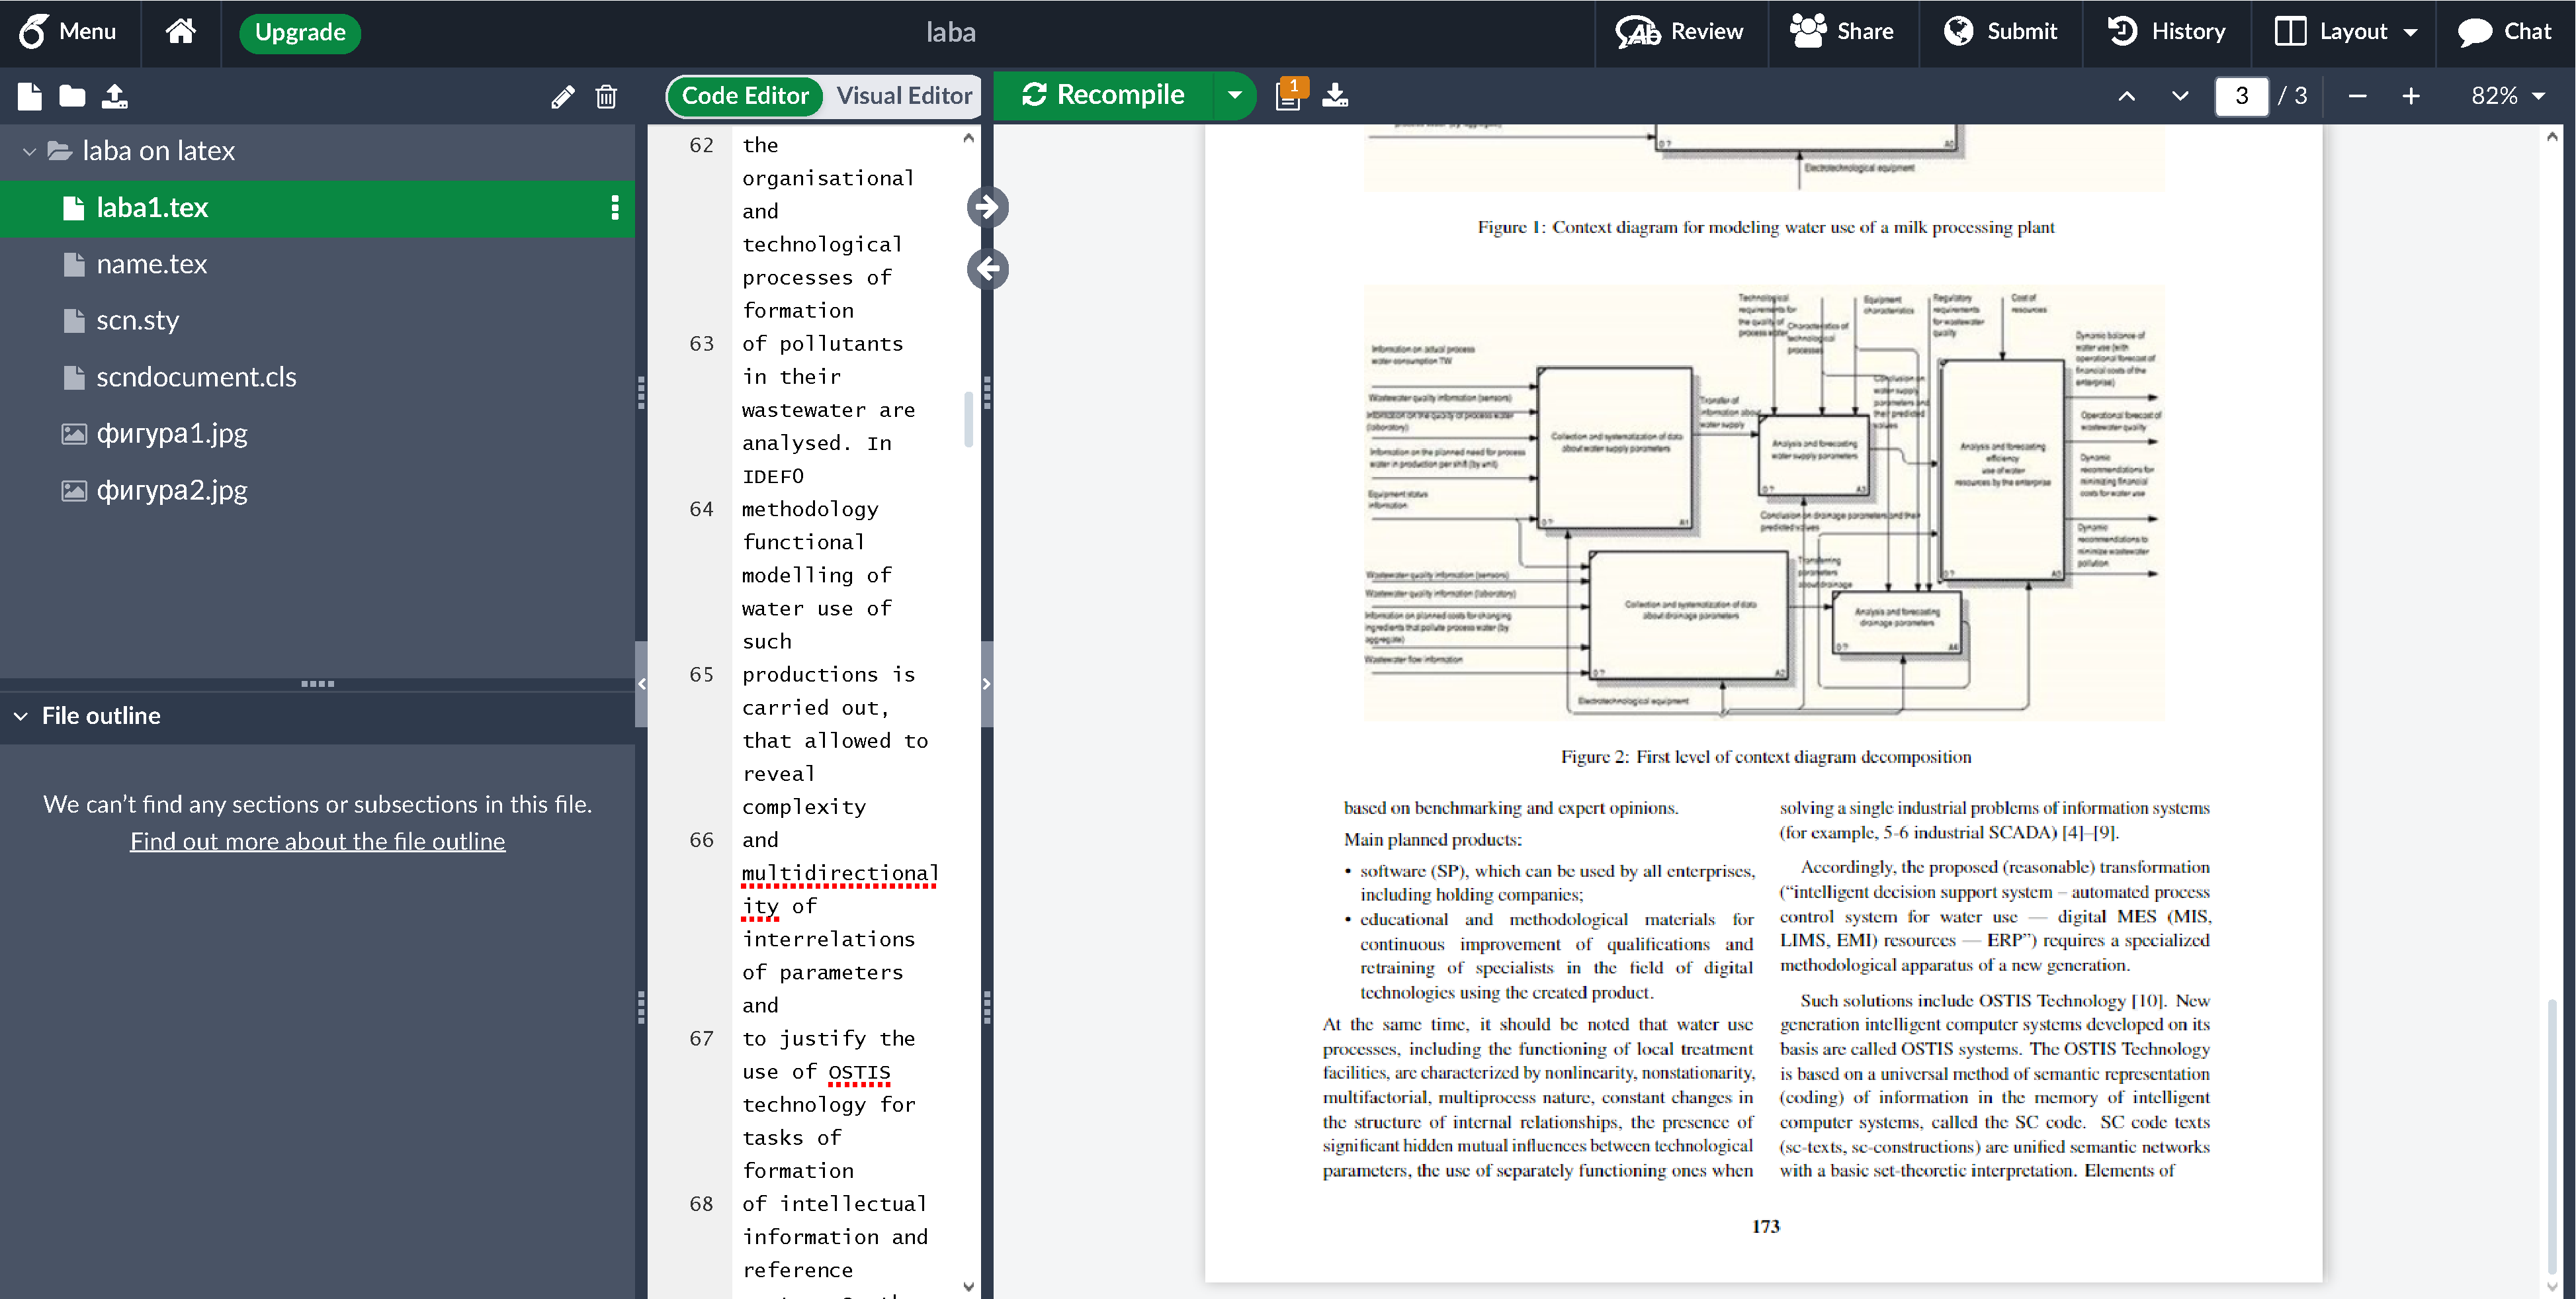
\includegraphics[width=0.9\linewidth]{images/picture3.png}
  \caption{\footnotesize Figure 3. Example of writing a conditional transition between two actions}
  \label{fig:picture3}
}

However, in order to constantly replenish the \textit{knowledge base} during the dialog process, it is necessary to extract \textit{knowledge} from the user’s messages and immerse them into the \textit{knowledge base.} For this purpose, the problem solver of the described system implements an action whose problem is to transform the natural-language text of messages into \textit{knowledge base} constructs.

Such a solution allows the system to better utilize knowledge for a more accurate and coherent answer,

\end{document}
